%! suppress = Unicode
%! Author = breandan
%! Date = 11/16/20

% Preamble
\documentclass[11pt]{article}

% Packages
\usepackage{amsmath}
\usepackage[pdf]{graphviz}
\usepackage{amssymb}
\usepackage{mathrsfs}

\usepackage{unicode-math}
\DeclareMathAlphabet{\mathcal}{OMS}{cmsy}{m}{n}
\usepackage{cancel}
\newcommand{\nDownarrow}{\ensuremath{\text{ }\cancel{\Downarrow}\text{ }}}
\usepackage{centernot}

\usepackage{pgfplots}
\usepgfplotslibrary{fillbetween}
\usetikzlibrary{patterns}
\pgfmathdeclarefunction{gauss}{2}{%
\pgfmathparse{1/(#2*sqrt(2*pi))*exp(-((x-#1)^2)/(2*#2^2))}%
}

\usepackage{adjustbox}
\usepackage{enumerate}
\usepackage{enumitem}
\usepackage{tikz-cd}
\usepackage{amsfonts}
%\usepackage{prooftrees}
\usepackage{bussproofs}
\usepackage{hyperref}
\renewcommand{\sectionautorefname}{\S}
\renewcommand{\subsectionautorefname}{\S}
\usepackage{natbib}
\usepackage{float}
\usepackage{xcolor}

\usepackage{algpseudocode}
\usepackage{algorithmicx}
\usepackage{sourcecodepro}
\usepackage{listings}
\usepackage{tikz-qtree}
\usepackage{amsthm}
\usepackage{bm}
\usetikzlibrary{bayesnet}
\usetikzlibrary{arrows}
\usepackage{caption}
\usepackage{subcaption}
\usetikzlibrary{backgrounds}

\newcommand{\E}{\mathbb{E}}
\newcommand{\Var}{\mathrm{Var}}
\newcommand{\Cov}{\mathrm{Cov}}

\newcommand{\CompOrder}{\mathcal{O}}
\def\graphspace{\mathbf{G}}
\def\Uniform{\mbox{\rm Uniform}}
\def\Gaussian{\mbox{\rm Gaussian}}
\def\Bernoulli{\mbox{\rm Bernoulli}}
\def\Dirichlet{\mbox{\rm Dirichlet}}

\usepackage{mathtools}% superior to amsmath
\usepackage{tikz}
\usepackage{graphicx}


\title{Pattern Recognition in Procedural Knowledge}
\author{Breandan Considine}
\date{\today}

% Document
\begin{document}
    \maketitle

    \tableofcontents
    \pagebreak


    \section{Introduction}

    Historically, most knowledge was stored as natural language. A growing portion is now \textit{code}~\citep{allamanis2018survey}. The majority of code is procedural knowledge, written by a human and intended to operate a machine. Though it shares many statistical properties in common with natural language~\citep{hindle2012naturalness}, code has a well-defined grammar and unambiguous semantics~\citep{pierce2010software}. We can use these properties to precisely reason about operational or procedural correctness.

    Prior work explored differentiable programming~\citep{considine2019programming}. Differentiability plays a key role in learning, but does not provide the necessary vocabulary to describe human knowledge. In order to capture human knowledge and begin to reason as humans do, programs must be able to express the concept of \textit{uncertainty}. In this work, we propose a set of tools and techniques for reasoning about uncertainty in the form of \textit{procedural knowledge}. We define procedural knowledge as a set of routines representing abstract data transformations and how to realize them on a physical computer.

    To reason about procedural knowledge, we must first define what it means for two procedures to be equal. Although equality is known to be undecidable in most languages, various equivalence tests and semi-decision procedures have been developed. For example, we could rewrite said procedures~\citep{baader1999term}, compare them in various contexts~\citep{felleisen1990expressive}, and simulate or execute them on various input data~\citep{chen2020metamorphic} so as to ascertain their exact relationship.

    In practice, exact equality is too rigid to operationalize. A more useful theory would allow us to compare two similar procedures in the presence of naturally-arising stochasticity. What is the probability of observing local variations? How are those observations related? And how do local variations affect global behavior? In order to correctly pose these questions and begin to answer them, we must be able to reason probabilistically.

    Graphs are a natural representation for both procedural knowledge~\citep{allamanis2017learning} and probabilistic reasoning~\citep{pearl2014probabilistic}, both enabling a large class of useful data transformations and vastly simplifying their implementation on physical machinery. Depending on the author's perspective, it is possible to view the evaluation of these routines as either operating a stateful machine, reducing a symbolic expression or running a dynamical process on a dataflow graph.

    In this work, we will define exact and approximate equality and cover some deterministic and probabilistic algorithms for deciding it. We will then describe a few graph representations for encoding approximate procedural knowledge. Finally, we will discuss some opportunities for applying these ideas to search-based software engineering, in particular code search, vulnerability detection, fault localization and program repair.


    \section{From exact to approximate equality}\label{sec:definitions}

    Reason is the source of all human knowledge. In order to understand reason, we need to understand how concepts are related. Next to identity, one of the simplest relations is equality. Equality is like identity for objects that may differ in superficial ways, but are the same in all but name and appearance.

    For such a fundamental concept, the notation for equality is recklessly overloaded in mathematics and computer science. Depending on context, $x = y$ may denote: (1)~define $x$ to be $y$, (2)~$x$ and $y$ are the same, (3)~are $x$ and $y$ the same? (4)~$x$ and $y$ are exchangeable, (5)~assign $y$ to $x$, (6)~assign $x$ to $y$, among other peculiar programming idioms. If two expressions are equal, it should be possible to treat them in the same manner.

    But this convention does not always hold! Suppose we need to compute the derivative of a logical function with respect to its inputs. The trouble is, logical equality is not differentiable. Consider the Kronecker $δ$-function: %$δ_k: \mathbb{N}^2\rightarrow \mathbb{B}$:

    $$
    δ_k(x, y) :=
    \begin{cases}
        1 \text{ if } x \overset{?}{=} y, \\
        0 \text{ otherwise }\\
    \end{cases}
    $$

    When encountering $δ_k$, how should we represent its derivative? Since $\mathbb{B}$ is finite, $δ_k^{-1}(B\subset \mathbb{B})$ is not open, thus $δ_k$ is not continuous and $\nablaδ_k$ is undefined. Now consider the Dirac $δ$-function, which is defined as follows: %$δ_d: \mathbb{R}^2 \rightarrow \mathbb{R}$,

    $$
    \forall f \in \mathbb{R}^2 \rightarrow \mathbb{R}, \int_{\mathbb{R}^2} f(x,y)δ_d(x-a,y-b)d(x, y) \overset{Δ}{=} f(a,b)
    $$

    Unlike $\nablaδ_k$, it can be shown that $\nablaδ_d$ is well-behaved everywhere on $\mathbb{R}^2$. However we encounter an important distinction between intensional and extensional equality. Unlike elementary functions, there exist many functions which can only be described indirectly, e.g. a probability distribution on a set of measure zero. Nevertheless, these constructions are convenient abstractions for modeling many physical and computational processes.

    Neither $δ_k$ nor $\nablaδ_d$ are a satisfactory basis for logical equality. To allow a more flexible definition of the $\overset{?}{=}$ operator, we require a relation which approximates the logical properties of $δ_k$, but can be made differentiable like $δ_d$. A more general notion is the concept of an \textit{equivalence relation} $\equiv$, a binary relation with the following logical properties:

    \begin{prooftree}
        \bottomAlignProof
        \AxiomC{}
        \UnaryInfC{$a \equiv a$}
        \noLine
        \UnaryInfC{}
        \noLine
        \UnaryInfC{\textit{Identity}}
        \DisplayProof
        \hskip 1.5em
        \bottomAlignProof
        \AxiomC{$a \equiv b$}
        \UnaryInfC{$b \equiv a$}
        \noLine
        \UnaryInfC{}
        \noLine
        \UnaryInfC{\textit{Symmetry}}
        \DisplayProof
        \hskip 1.5em
        \bottomAlignProof
        \AxiomC{$a \equiv b$}
        \AxiomC{$b \equiv c$}
        \BinaryInfC{$a \equiv c$}
        \noLine
        \UnaryInfC{}
        \noLine
        \UnaryInfC{\textit{Transitivity}}
        \DisplayProof
        \hskip 1.5em
        \bottomAlignProof
        \AxiomC{$a \equiv b$}
        \UnaryInfC{$f(a) \equiv f(b)$}
        \noLine
        \UnaryInfC{}
        \noLine
        \UnaryInfC{\textit{Congruence}}
    \end{prooftree}

    \pagebreak\subsection{Decidability}\label{sec:algorithms}

    To determine if two procedures are equal, we need a decision procedure. We list several high-level approaches for deciding exact and approximate equality in the deterministic and probabilistic setting in the table below:

    \bgroup
    \def\arraystretch{1.2}
    \begin{table}[H]
        \centering
        \begin{tabular}{c|l|l|}
            \cline{2-3} & \textbf{Deterministic} & \textbf{Probabilistic} \\ \hline
            \multicolumn{1}{|c|}{\textbf{Exact}} & \begin{tabular}[c]{@{}l@{}}
                                                       Type Checking\\ Model Checking
            \end{tabular} & \begin{tabular}[c]{@{}l@{}}
                                Variable Elimination\\Probabilistic Circuits
            \end{tabular} \\ \hline
            \multicolumn{1}{|c|}{\textbf{Approximate}} & \begin{tabular}[c]{@{}l@{}}
                                                             Software Testing\\Dynamic Analysis
            \end{tabular} & \begin{tabular}[c]{@{}l@{}}
                                Monte Carlo Methods\\Bayesian Networks
            \end{tabular} \\ \hline
        \end{tabular}
    \end{table}
    \egroup

    It is seldom the case that two semantically equal expressions are trivially equal: we must first perform some computation to establish their equality. In the exact setting, this procedure might be summarized as follows:

    \begin{enumerate}
        \item Rewrite: Either enumerate a set of equivalent expressions, or reduce the proposition into normal form if possible, then,
        \item Compare: Perform a computationally trivial (e.g. $\mathcal{O}(n)$) comparison.
    \end{enumerate}

    Unfortunately, exact equality is known to be undecidable in first~\cite{godel1929vollstandigkeit} and higher order theories~\cite{godel1931formal}. We know there can be no machine which accepts every equality and rejects every disequality in a universal language~\cite{turing1937computable}. By extension, any nontrivial property of partial functions is undecidable~\cite{rice1953classes}. %Equality between two elementary mathematical functions is undecidable~\cite{richardson1994identity}.

    %Is there any left hope? Yes! (Felleisen)

    Tractability may be related to, but is not contingent upon decidability. When decidable, equality may be intractable in practice, and languages where equality is undecidable may have decidable fragments. But even when exact equality is intractable, we may be able to construct a probabilistic decision procedure (PDP) or semidecision procedure (SDP) terminating for all practical purposes. The latter approaches fall into two broad categories:

    \begin{itemize}
        \item Execute: Evaluate the program by running it on a small set of inputs
        \item Sample: Build a probabilistic model and sample from its distribution
    \end{itemize}

    In the following section, we will introduce a few compatible theories corresponding to intensional and extensional equality, then build on those definitions to include recent approaches to exact and approximate equality in the determinsitic and probabilistic setting. In so doing, we will see there is a delicate tradeoff between complexity, sensitivity and specificity.

%    Mathematics is often a useful approximation of reality, but many mathematical concepts are impossible to realize. This is due to two problems:
%
%    \begin{enumerate}
%        \item intrinsic: the mechanics of the system are intrinsically unsound or impossible to mechanize. How do we encode $\lim_{x \rightarrow \infty}$?
%        \item extrinsic: all descriptions (epistemic) and observations (alleoteric) are approximate and this error can compound quickly.
%    \end{enumerate}


%    But can we organize mathematical knowledge as a decision tree? (Rich)

%    Still, we can answer many questions exactly. If we restrict the reasoning system to incomplete queries, we can be consistent.

    \subsection{Intensional equivalence}\label{subsec:in-eq}

    Let $Ω \subseteq \mathcal{F} \times \mathcal{F}$ be a relation on representable functions which are closed under composition. We say two representations $f, g \in \mathcal{X} \rightarrow \mathcal{Y}$ are intensionally equal under $Ω$ if we can establish that $g \in Ω^n(f)$ for some $n \in \mathbb{N}$.

    \begin{prooftree}
        \AxiomC{$f, g: \mathcal{X \rightarrow Y} \in Γ^0_{g}$}
        \RightLabel{\textsc{Init}}
        \UnaryInfC{$Γ^0_{g} \vdash \{f\}, \{(f, f)\}$}
%        \UnaryInfC{\textit{Commutivity}}
        \DisplayProof
        \hskip 1em
        \AxiomC{$Γ^{n}_{g} \vdash E \subseteq \mathcal{F}, G \subseteq E \times E$}
        \RightLabel{\textsc{Sub}}
        \UnaryInfC{$Γ^{n+1}_{g} \vdash \bigcup\limits_{\substack{e \in E\\\sigma \in Ω}}e'\leftarrow e[\sigma_1\rightarrow\sigma_2], (e, e')$}
        \DisplayProof
        \vskip 1em
        \AxiomC{$Γ^n_{g} \vdash E, G$}
        \AxiomC{$g \in E$}
        \RightLabel{\textsc{Eq}}
        \BinaryInfC{$Γ^n_{g} \vdash f \equiv_Ω g$ by $G^{-n}(g)$}
        \DisplayProof
        \hskip 1em
        \AxiomC{$Γ^n_{g} \vdash E$}
        \AxiomC{$Γ^{n+1}_{g}\vdash E$}
        \AxiomC{$g\notin E$}
        \RightLabel{\textsc{Neq}}
        \TrinaryInfC{$Γ^{n+1}_{g} \vdash f \not\equiv_Ω g$}
    \end{prooftree}

    \noindent For example, suppose we are given $f: \{a, b, c\} \mapsto a b c, g: \{a, b, c\} \mapsto c b a$ and $Ω := \{(a, a), (ab, ba)\}$. Indeed, $\textsc{Eq}[f, g]$ can be established as follows:

    \vspace{-10pt}\begin{prooftree}
        \def\fCenter{\ := \ }
        \Axiom$f \fCenter abc, \text{ } g := cba \in Γ_g^0$
        \def\fCenter{\ \vdash\ }
        \RightLabel{\textsc{Init}}
        \UnaryInf$Γ^0_{g} \fCenter \{abc\}, \{(abc, abc)\}$
        \RightLabel{\textsc{Sub}}
        \UnaryInf$Γ^1_{g} \fCenter \{\ldots, bac, acb\}, \{\ldots, (abc, bac), (abc, acb)\}$
        \RightLabel{\textsc{Sub}}
        \UnaryInf$Γ^2_{g} \fCenter \{\ldots, bca, cab\}, \{\ldots, (bac, bac), (acb, acb), (bac, bca), (acb, cab)\}$
        \RightLabel{\textsc{Sub}}
        \UnaryInf$Γ^3_{g} \fCenter \{\ldots, \mathbf{cba}\}, \{\ldots, (bca, bca), (cab, cab), (cab,\textbf{cba})\}$
        \RightLabel{\textsc{Eq}}
        \UnaryInf$Γ^3_{g} \fCenter f \equiv_Ω g\text{ by } G^{-3}(g:=cba) = \{f := abc\}$
    \end{prooftree}

    \noindent We can visualize $G$ as a directed graph, omitting all loops. Notice how each path converges to the same term, a property known as $\textit{strong confluence}$.

    \hspace{12pt}\digraph[scale=0.5]{abcint}{
    node[ fontname="CMU Classical Serif" fontsize=20 ];
    edge[ fontname="CMU Classical Serif" fontsize=18 ];
    rankdir=LR;
    len=3;
    node [shape=Mrecord];

    a [ label="abc"; ]
    b [ label="bac"; ]
    c [ label="acb"; ]
    d [ label="bca"; ]
    e [ label="cab"; ]
    f [ label="cba"; ]

%    a -> a [label="Σ₀"]
    a -> b [label=<Ω<SUB>1</SUB>> minlen=2]
    a -> c [label=<Ω<SUB>1</SUB>> minlen=2]
    b -> d [label=<Ω<SUB>1</SUB>> minlen=2]
    c -> e [label=<Ω<SUB>1</SUB>> minlen=2]
    e -> f [label=<Ω<SUB>1</SUB>> minlen=2]
    d -> f [label=<Ω<SUB>1</SUB>> minlen=2]
    }

    \noindent Let us suppose $|\mathcal{X}|, |Ω^*| \in \mathbb{N}$ and consider the complexity of establishing $\textsc{Eq}[f, g], \forall f \equiv_Ω g \in \mathcal{X} \rightarrow \mathcal{Y}$. It can be shown the above procedure requires:

    $$\mathcal{O}_{\textsc{Eq}} = \underset{i \leq n}{\text{max }}\underset{n}{\text{argmin}}\{|G| \mid Γ^i_{g} \vdash G, Γ_{g}^n = Γ_{g}^{n+1}\}$$ % \text{, or } \Theta_{\textsc{Eq}}(|\mathcal{X}|!) \text{ for } Ω.$$

    \noindent Assuming termination, $\mathcal{O}_{\textsc{Eq}} = \Theta_{\textsc{Neq}}$ although $\mathbb{E}[\Theta_\textsc{Eq}|f \equiv g]$ is more tractable. However termination is not necessarily guaranteed, e.g. $Ω' := \{(a, 1a)\}$. Equality and termination under arbitrary $Ω$ are known to be undecidable~\citep{baader1999term}.

    \subsection{Computational equivalence}\label{subsec:comp-eq}

    Clearly, the procedure defined in \S~\ref{subsec:in-eq} is highly sensitive to $|\mathcal{X}|$ and $Ω$. While equality may be tractable, disequality is definitely an obstacle. In the computational setting, we will see the opposite holds, ceteris paribus. %Two values $r, r': \mathcal{Y}$ share a normal form in which equality is trivial.

    \begin{prooftree}
        \AxiomC{$fg: \mathcal{X} \rightarrow \mathcal{Y}, Ω: \{\mathcal{X}\rightarrow \mathcal{Y}\}\rightarrow \mathcal{Y} \in Γ$}
        \RightLabel{\textsc{Inv}}
        \UnaryInfC{$Γ \vdash fg(Ω) \Downarrow f(Ω) \cdot g(Ω)$}
        \DisplayProof
        \hskip 1em
        \AxiomC{$Γ \vdash f$}
        \AxiomC{$Γ \vdash Ω$}
        \RightLabel{\textsc{Sub}}
%        \AxiomC{$i: \mathcal{X}$}
        \BinaryInfC{$Γ \vdash f(Ω) \Downarrow Ω[f]$}
        \DisplayProof
        \vskip 1em
        \AxiomC{$Γ, Γ' \vdash f(Ω) \Downarrow g(Ω) \text{ } \forall Ω$}
        \RightLabel{\textsc{Eq}}
        \UnaryInfC{$Γ, Γ' \vdash f \equiv g$}
        \DisplayProof
        \hskip 1em
        \AxiomC{$Γ, Γ' \vdash \exists Ω \mid f(Ω) \nDownarrow g(Ω) $}
        \RightLabel{\textsc{Neq}}
        \UnaryInfC{$Γ, Γ' \vdash f \not\equiv g$ by $Ω$}
    \end{prooftree}

    % big step semantics
%    Extensional equality asks``Do $f_1$ and $f_2$ behave in the same way over all inputs?''
    \noindent \textsc{Sub} loosely corresponds to $\eta$-reduction in the untyped $\lambda$-calculus, however $f \notin Ω$ is disallowed and we assume all variables are bound by \textsc{Inv}. Let us consider $f: \{a, b, c\}\mapsto abc, g: \{a, b, c\} \mapsto ac$ under $Ω:=\{(a, 1), (b, 2), (c, 2)\}$:

    %If we test $\hat i \in {-2, -1, 0, 1, \ldots}$, we have $f_1(-2)=f_2(-2)$, $f_1(-1)=f_2(-1)$, $f_1(0)=f_2(0)$, $f_1(1) \neq f_2(1)$. Once we detect an $f_1(\hat i) \neq f_2(\hat i)$, we can halt immediately.

    \vspace{-10pt}\begin{prooftree}
        \def\fCenter{\ :=}
        \def\defaultHypSeparation{\hskip -1.1in}
        \Axiom$f\fCenter abc, Ω:=\{(a, 1), (b, 2), (c, 2)\} \in Γ$
        \def\fCenter{\ \vdash\ }
        \RightLabel{\textsc{Inv}}
        \UnaryInf$Γ \fCenter a(Ω)\cdot bc(Ω)$
        \RightLabel{\textsc{Sub}}
        \UnaryInf$Γ \fCenter 1\cdot bc(Ω)$
        \RightLabel{\textsc{Inv}}
        \UnaryInf$Γ \fCenter 1\cdot b(Ω)\cdot c(Ω)$
        \RightLabel{\textsc{Sub}}
        \UnaryInf$Γ \fCenter 2\cdot c(Ω)$
        \RightLabel{\textsc{Sub}}
        \UnaryInf$Γ \fCenter f(Ω) \Downarrow 4$
        \def\fCenter{\ :=}
        \Axiom$g\fCenter ac, Ω:=\{(a, 1), (b, 2), (c, 2)\} \in Γ'$
        \def\fCenter{\ \vdash\ }
        \RightLabel{\textsc{Inv}}
        \UnaryInf$Γ' \fCenter a(Ω)\cdot c(Ω)$
        \RightLabel{\textsc{Sub}}
        \UnaryInf$Γ' \fCenter 1\cdot c(Ω)$
        \RightLabel{\textsc{Sub}}
        \UnaryInf$Γ' \fCenter g(Ω) \Downarrow 2$
        \RightLabel{\textsc{Neq}}
        \BinaryInfC{$Γ, Γ' \vdash f \not\equiv g$ by $Ω :=\{(a, 1), (b, 2), (c, 2)\}$}
    \end{prooftree}

    \noindent We can view the above process as acting on a dataflow graph, where \textsc{Inv} backpropagates $Ω$, and \textsc{Sub} returns concrete values $\mathcal{Y}$, here depicted on $g$:

    \hspace{-30pt}\digraph[scale=0.5]{abcext0}{
    node[ fontname="CMU Classical Serif" fontsize=20 ];
    edge[ fontname="CMU Classical Serif" fontsize=18 ];
    rankdir=LR;
    len=3;
    node [shape=Mrecord];

    f [ label="g"; ]
    a [ label="a"; ]
    c [ label="c"; ]
    d [ label="·"; ]

%    a -> a [label="Σ₀"]
    f -> d [label="Ω"]
    d -> a [label="Ω"]
    d -> c [label="Ω"]
    }\hspace{-20pt}\digraph[scale=0.5]{abcext1}{
    node[ fontname="CMU Classical Serif" fontsize=20 ];
    edge[ fontname="CMU Classical Serif" fontsize=18 ];
    rankdir=LR;
    len=3;
    node [shape=Mrecord];

    f [ label="g"; ]
    a [ label="a"; ]
    c [ label="c"; ]
    d [ label="·"; ]

%    a -> a [label="Σ₀"]
    d -> f [label="𝓨"]
    a -> d [label="𝓨"]
    c -> d [label="𝓨"]
    }

    \noindent Assuming $f, g \sim P(\mathcal{F}), Ω \overset{iid}{\sim} P_\textsc{Test}(Ω \mid f \not\equiv g)$ yields a fixed but unknown distribution, $P_\textsc{Neq}(Ω) = P(f(Ω) \nDownarrow g(Ω) \mid f \not\equiv g)$. Let $\Theta_\textsc{Inv} = 1$ for all $f, Ω$. The complexity of certifying $\textsc{Neq}$ in $n$ trials follows a geometric distribution:

    \vspace{-10pt}$$\Theta_\textsc{Neq} \sim (1 - P_\textsc{Neq}(Ω))^nP_\textsc{Neq}(Ω) \text{ with } \mathop{\mathbb{E}}[\Theta_\textsc{Neq}] = (1-P_\textsc{Neq}(Ω))P_\textsc{Neq}(Ω)^{-1}$$

    \noindent Although a single witness $Ω$ s.t. $f(Ω) \nDownarrow g(Ω)$ is sufficient for disequality, this procedure may be intractable depending on $|\mathcal{X}|, P_\textsc{Neq}(Ω)$ and $\Theta_{\textsc{Inv}}$. Other fuzzing methods for selecting $Ω$ based on the structure of $f$ are also possible.

%    We can test using property-based / metamorphic testing. Some strategies:

%    Isomorphism testing

%    Metamorphic testing


    \pagebreak\subsection{Observational equivalence}

    As presented, both intensional (\S~\ref{subsec:in-eq}) and computational (\S~\ref{subsec:comp-eq}) equivalence require an external definition of equality to satisfy. One solution to this problem known as \textit{observational equivalence}~\cite{morris1969lambda} allows a language $\mathcal{L}$ to implement an internal mechanism to verify equality. Given $\mathcal{L}$, a term $t$, and one-hole context $C[\![\cdot]\!]$, our job is to check for termination: if $C[\![t]\!]$ is both well-defined and halts, we write $C[\![t]\!]\Downarrow$, otherwise $C[\![t]\!]\Uparrow$.

    \begin{prooftree}
        \AxiomC{$Γ \vdash C[\![t]\!]\Downarrow \iff C[\![t']\!]\Downarrow$ $\forall$ $C[\![\cdot]\!] \in \mathcal{L}$}
        \RightLabel{\textsc{Eq}}
        \UnaryInfC{$Γ \vdash t \equiv_{\mathcal{L}} t'$}
        \DisplayProof
        \vskip 1em
        \AxiomC{$Γ \vdash \exists C[\![\cdot]\!]\in \mathcal{L} \mid C[\![t]\!]\Uparrow $ and $ C[\![t']\!]\Downarrow$, or $C[\![t]\!]\Downarrow $ and $ C[\![t']\!]\Uparrow$}
        \RightLabel{\textsc{Neq}}
        \UnaryInfC{$Γ \vdash t \not\equiv_{\mathcal{L}} t'$ by $C[\![\cdot]\!]$}
    \end{prooftree}

%    http://www.cs.ox.ac.uk/people/samuel.staton/papers/fossacs-2019.pdf
%    http://users.ox.ac.uk/~scro3229/documents/birmingham-talk.pdf

    We can think of this definition as dual to computational equivalence: instead of searching for inputs which distinguish functions, we search for contexts which distinguish terms, or a proof that no such context exists. Two terms $t$ and $t'$ are contextually equivalent with respect to $\mathcal{L}$ if we can prove that for all contexts $C[\![\cdot]\!]$ in $\mathcal{L}$, $C[\![t]\!]$ halts if and only if $C[\![t']\!]$ halts -- if no such proof can be found, the test is inconclusive. While this definition does not admit a decision procedure, many promising SDPs exist.

%    $P(w_t = a | w_{t-1}, w_{t-2}\ldots, w_{t+1}, w_{t+2}, \ldots)\overset{?}{\approx} P(w_t = b | w_{t-1}, w_{t-2}\ldots, w_{t+1}, w_{t+2}, \ldots)$

%    We can define semantic equality in our setting using word embeddings.

    \subsection{Approximate equivalence}\label{sec:ap-eq}

    Though precise, boolean equality is far too rigid for many applications. The spaces involved either lack formal semantics or are intractable to verify, leaving decidability out of reach. We can relax this definition by introducing a generalized equivalence relation for reasoning on continuous spaces, called a \textit{distance metric}, $δ: \mathcal{Z}\times\mathcal{Z}\rightarrow\mathbb{R}_{\geq 0}$. This has the following logical properties:

    \begin{prooftree}
        \bottomAlignProof
        \AxiomC{$δ(a, b) = 0$}
        \UnaryInfC{$a \equiv_δ b$}
        \noLine
        \UnaryInfC{}
        \noLine
        \UnaryInfC{\textit{Definiteness}}
        \DisplayProof
        \hskip 1.5em
        \bottomAlignProof
        \AxiomC{$δ(a, b)$}
        \UnaryInfC{$δ(b, a)$}
        \noLine
        \UnaryInfC{}
        \noLine
        \UnaryInfC{\textit{Symmetry}}
        \DisplayProof
        \hskip 1.5em
        \bottomAlignProof
        \AxiomC{$a$}
        \AxiomC{$b$}
        \AxiomC{$c$}
        \TrinaryInfC{$δ(a, c) \leq δ(a, b) + δ(b, c)$}
        \noLine
        \UnaryInfC{}
        \noLine
        \UnaryInfC{\textit{Triangularity}}
    \end{prooftree}

    \noindent A \textit{kernel function} $Δ: (\mathcal{X}\rightarrow\mathcal{Y})^2\rightarrow \mathbb{R}_{\geq 0}$ can be defined as a metric on $\mathcal{Z}$ with some additional structure. Specifically for every kernel function, there exists a feature map $\varphi: (\mathcal{X}→\mathcal{Y}) → \mathcal{Z}$ such that $Δ: (f, g) \mapsto \left<\varphi(f), \varphi(g)\right>$. Given a feature map $\symbf\varphi: \mathbb{R}^m → \mathbb{R}^n$, constructing a kernel corresponds to finding $\Delta \in \mathbb{R}^{m \times m}$ symmetric PSD, i.e. $\Delta^\intercal = \Delta$, and $0 \leq \mathbf{x}^\intercal \Delta \mathbf{x}$ for all $\mathbf{x} \in \mathbb{R}^m$~\cite{mercer1909functions}. Consider the complexity of evaluating the inner product $\left<\symbf\varphi(f), \symbf\varphi(g)\right>$ in feature space. The computational benefit of a kernel becomes apparent when $m \ll n$. Rather than applying $\symbf\varphi$, then evaluating $\left<f^\intercal\symbf\varphi, g^\intercal\symbf\varphi\right>$, we may apply $\Delta(f, g)$ directly for a $\Theta(m^2 - n^2)$ speedup. Known as the \textit{kernel trick}, this shortcut may be easier to see categorically, where $f, g: \mathcal{X}→\mathcal{Y}$.

    \[\begin{tikzcd}
          (\mathcal{X→\mathcal{Y}})^2 \arrow{r}{\varphi} \arrow[labels=below left]{dr}{\Delta} & \mathcal{Z}\times\mathcal{Z} \arrow{d}{\left<\cdot, \cdot\right>} \\
          & \mathbb{R}_{\geq 0}
    \end{tikzcd}
    \]

    \noindent By planting a single valid kernel $\Delta$, one can grow a tree of kernel functions $▲ \subset (\mathcal{X}→\mathcal{Y})^2 → \mathbb{R}_{\geq 0}$ which may be described by the following grammar:

    % https://papers.nips.cc/paper/2000/file/4e87337f366f72daa424dae11df0538c-Paper.pdf
    % https://www.stat.berkeley.edu/~bartlett/courses/2014spring-cs281bstat241b/lectures/20-notes.pdf#page=17
    % https://people.eecs.berkeley.edu/~jordan/kernels/0521813972c03_p47-84.pdf#page=29
%    http://www.cs.cmu.edu/~aarti/Class/10701_Spring14/slides/kernel_methods.pdf#page=38

    \begin{prooftree}
        \bottomAlignProof
        \AxiomC{$Δ \in ▲, k \in \mathbb{R}_{\geq 0}$}
        \UnaryInfC{$kΔ \in ▲$}
        \DisplayProof
        \hskip 0.6em
        \bottomAlignProof
        \AxiomC{$Δ_{1, 2} \in ▲$}
        \UnaryInfC{$Δ_1 + Δ_2 \in ▲$}
        \DisplayProof
        \hskip 0.6em
        \bottomAlignProof
        \AxiomC{$Δ_{1, 2} \in ▲$}
        \UnaryInfC{$Δ_1Δ_2 \in ▲$}
        \DisplayProof
        \hskip 0.6em
        \bottomAlignProof
        \AxiomC{$Δ \in ▲, f \in (^*→\mathcal{Z})^2$}
        \UnaryInfC{$Δ\circ f \in ▲$}
    \end{prooftree}

    \noindent Some elementary kernel functions for various datatypes are given below:

    %, we can construct the corresponding kernel as follows...

    \bgroup
    \def\arraystretch{1.7}
    \begin{center}
        \begin{tabular}{|c|c|c|}
            \cline{2-3}
            \multicolumn{1}{c|}{} & $\Delta(f,g)$ & $\varphi(x) $\\\hline
            % http://www.cs.rpi.edu/~stewart/lec23-post/kernels.pdf#page=14
%            https://people.eecs.berkeley.edu/~jordan/kernels/0521813972c09_p291-326.pdf#page=5
            Polynomial & $\big(\mathbf{f}^\intercal\mathbf{g} + r\big)^{q}$ & $\Big[\sqrt{{q \choose \mathbf{n}}r^{n_0}}\prod_{k} x_k^{n_k}\Big]^\intercal_{\mathbf{n} \in \{\mathbf{n}\mid  \mathbf{1^\intercal n} = q\}}$ \\ \hline
            % https://vikas.sindhwani.org/RandomLaplace.pdf#page=3
            % https://www.csie.ntu.edu.tw/~cjlin/talks/kuleuven_svm.pdf#page=11
            Gaussian RBF & $e^{-{\frac {\|\mathbf{f} -\mathbf{g} \|^{2}}{2\sigma ^{2}}}}$ & $e^{-γx^2} \Big[1, \sqrt{\frac{(2γ)^i}{i!}}x^i\Big]^\intercal_{i\in (0, \text{dim}(x)-1]}$ \\ \hline
%            https://people.eecs.berkeley.edu/~jordan/kernels/0521813972c09_p291-326.pdf#page=4
            Subset & $\prod_{i = 1}^n (f_i g_i + 1)$ & $[\varphi_\textsc{Poly}(x)_A]^\intercal_{A\subseteq [1, n]}$\\ \hline
%            https://people.eecs.berkeley.edu/~jordan/kernels/0521813972c11_p344-396.pdf
%            https://people.eecs.berkeley.edu/~jordan/kernels/0521813972c11_p344-396.pdf#page=8
            Substring & $\sum_{\sigma \in Σ^*}(f * σ)(g * σ)$ & $|\{i \mid \sigma = x_{i..(i+|σ|)}\}|$ \\ \hline
            Subtree~\cite{shervashidze2009fast} & $\Delta_\textsc{WL}(f, g)$ &
            \[ \begin{cases}
                   δ_k(t, x) & t \overset{?}{=} x\\
                   \varphi_t(\overset{\leftarrow}{x}) + \varphi_t(\overset{\rightarrow}{x}) & \text{otherwise.} \\
            \end{cases}
            \] \\ \hline
%            https://people.eecs.berkeley.edu/~jordan/kernels/0521813972c11_p344-396.pdf#page=44
%            https://papers.nips.cc/paper/2009/file/0a49e3c3a03ebde64f85c0bacd8a08e2-Paper.pdf#page=4
%            https://www.cs.mcgill.ca/~wlh/grl_book/files/GRL_Book.pdf#page=22
            Subgraph~\citep{hamilton2020graph} & $\Delta_\textsc{SS}\big(\varphi^{(h)}(f), \varphi^{(h)}(g)\big)$ & $\textsc{Hash}\big(\{\{\varphi^{(i - 1)}(u) \forall u \in \mathcal{N}(x)\}\}\big)$ \\ \hline
        \end{tabular}
    \end{center}
    \egroup

    \noindent An \textit{approximate equivalence relation} is a binary relation $\mathcal{A} \subset \mathcal (\mathcal X → \mathcal Y)^2$,~ e.g. $f \approx_{d} g \Leftrightarrow \mathbb \Delta(f, g) \leq d$. Given a dataset $X := [x^{(i)}]_{i=1}^n$, $Y := [f(x^{(i)})]_{i=1}^n$ and a program $g: \mathcal{X} → \mathcal{Y}$, we could use the extensional approach to evaluate $\Delta_X: (f, g) \mapsto \Delta_Y(Y, [g(x^{(i)})]_{i=0}^n)$ directly. Alternately, given an intensional descriptor $\varphi_θ(\cdot): (\mathcal X → \mathcal Y) → \mathcal Z$ we could construct a synthetic kernel $\Delta_θ: (f, g) \mapsto \left<\varphi_θ(f), \varphi_θ(g)\right>$, seeking $θ^* = \text{argmin}_θ\big(\Delta_θ(f, g) - \Delta_X(f, g)\big)^2$ over $f, g \overset{iid}{\sim} P(\mathcal X → \mathcal Y), X \overset{iid}{\sim} P(\mathcal X^n)$ via gradient descent. The problem then becomes: how do we match the distribution of naturally-arising programs?

%    It is often the case we are given a dataset $P_{\text{Train}}, P_{\text{Test}}: (X \times Y)^n$ sampled from an inaccessible distribution $P^{(1..n)} \overset{iid}{\sim} P_\text{Gen}(X, Y)$, and want to compare a deterministic computer program $\hat p: X \times \Theta → Y$ approximating $P_\text{Gen}$ to detect errors with respect to that dataset. One mechanism for doing so can be described as follows:...

%    \begin{prooftree}
%        \AxiomC{$Γ \vdash f \circ g, f: Z → Y, g: X → Z, B: := P_\text{Train}[i]$}
%        \RightLabel{\textsc{SGD}}
%        \UnaryInfC{$Γ \vdash t \equiv_{\mathcal{L}} t'$}
%        \DisplayProof
%        \vskip 1em
%%        \AxiomC{$Γ \vdash \exists C[\![\cdot]\!]\in \mathcal{L} \mid C[\![t]\!]\Uparrow $ and $ C[\![t']\!]\Downarrow$, or $C[\![t]\!]\Downarrow $ and $ C[\![t']\!]\Uparrow$}
%%        \RightLabel{\textsc{ERM}}
%%        \UnaryInfC{$Γ \vdash t \not\equiv_{\mathcal{L}} t'$ by $C[\![\cdot]\!]$}
%    \end{prooftree}


    \pagebreak\subsection{Probabilistic equivalence}\label{sec:pr-eq}

    So far, we have seen various notions of exact and approximate equivalence. However, what is needed is a way to quantify the probability a certain output is produced, or the likelihood of observing a representable function in the wild, given some prior knowledge. To do this properly, we need a language for propagating uncertainty through a computation. Probabilistic inference is one such framework for reasoning about uncertainty. In this section, we define a denotational and operational semantics for probabilistic inference. \\

    \noindent Let $E$ be a set of \textit{events} and $S$ a set of subsets of $E$. A \textit{probability distribution} is a function $P: S \times \Sigma \rightarrow \mathbb{R}^{+}$, which satisfies the Kolmogorov~\cite{kolmogorov1933grundbegriffe} axioms:

    \begin{itemize}
        \itemsep-1em
        \item [(3)] $P(S = s) \in \mathbb{R}^{+}, \forall s \in S$. ($S \overset{?}{=} s$ is usually written $S = s$ for brevity.) \\
        \item [(4)] $P(E) := 1$. ($P(S = E)$ may be shortened to $P(E)$ for brevity.) \\
        \item [(5)] $P(X \cup Y) := P(X) + P(Y), \forall X \cap Y = \varnothing$.
    \end{itemize}

    \noindent Given a distribution over a set $X$, we can \textit{sample} from it to produce a single element from that set, a \textit{random variable}:

\begin{prooftree}
\AxiomC{$\Gamma \vdash P(X): X \times \Sigma \rightarrow \mathbb{R}^{+}$}
\AxiomC{$\Gamma \vdash x \sim P(X)$}
\RightLabel{Sample}
\BinaryInfC{$\Gamma \vdash x: (X \times \Sigma \rightarrow \mathbb{R}^{+}) \leadsto X$}
\end{prooftree}

%We can assign a probability distribution to a variable, by \textit{sampling} from it. As we increase the sample size, the distribution of values will converge to the true distribution.
%
%$$
%d \sim \mathcal{D}
%$$

\noindent The \textit{joint}, $P(X, Y)$, is a distribution over the product of two sets, $X \times Y$:

\begin{prooftree}
\AxiomC{$\Gamma \vdash P(X): X \times \Sigma \rightarrow \mathbb R^{+}$}
\AxiomC{$\Gamma \vdash P(Y): Y \times \Sigma \rightarrow \mathbb R^{+}$}
\RightLabel{Join}
\BinaryInfC{$\Gamma \vdash P(X, Y): X \times Y \times \Sigma \rightarrow \mathbb R^{+}$}
\end{prooftree}

\noindent Given a joint $P(X, Y)$, if we observe an event $y: Y$, this observation is called \textit{conditioning} and the resulting distribution over $X$, a \textit{conditional distribution}:

% https://www.cambridge.org/core/services/aop-cambridge-core/content/view/819623B1B5B33836476618AC0621F0EE/9781108488518AR.pdf/Foundations_of_Probabilistic_Programming.pdf?event-type=FTLA#page=325
\begin{prooftree}
\AxiomC{$\Gamma \vdash P(X, Y): X \times Y \times \Sigma \rightarrow\mathbb{R}^+$}
\AxiomC{$\Gamma \vdash y: Y$}
\RightLabel{Cond}
\BinaryInfC{$\Gamma \vdash P(X \mid Y = y): X \times \Sigma \rightarrow\mathbb{R}^+$}
\end{prooftree}

\noindent In general, conditioning is order-dependent. Given a conditional distribution and its prior, to exchange the order of conditioning, we can use Bayes rule:

\begin{prooftree}
\AxiomC{$\overbrace{P(X \mid Y)}^{\text{Likelihood}}$}
\AxiomC{$\overbrace{P(Y)}^{\text{Prior}}$}
\RightLabel{Bayes}
\BinaryInfC{$\underbrace{P(Y \mid X) \propto}_{\text{Normalize}} \underbrace{P(X \mid Y)}_{\text{Observe}}\underbrace{P(Y)}_{\text{Sample}}$}
\end{prooftree}

\noindent When a conditional distribution $P(X \mid Y)$ does not depend on its prior, the events are said to be \textit{independent}. Equivalently, if two distributions $P(X)$ and $P(Y)$ are multiplied to form a joint distribution $P(X, Y)$, we may also conclude that $X$ and $Y$ are independent events:

\begin{prooftree}
\AxiomC{$P(X \mid Y) \equiv P(X)$}
\RightLabel{Indep}
\UnaryInfC{$X \perp Y$}
\DisplayProof
\hskip 1.5em
\AxiomC{$P(X, Y) \equiv P(X)P(Y)$}
\RightLabel{Factor}
\UnaryInfC{$X \perp Y$}
\end{prooftree}

\noindent When two conditionals $P(X \mid Z)$, $P(Y \mid Z)$ are multiplied to form a joint distribution $P(X, Y \mid Z)$, $X$ and $Y$ are \textit{conditionally independent given $Z$}:

\begin{prooftree}
\AxiomC{$P(X,Y \mid Z) \equiv P(X \mid Z)P(Y \mid Z)$}
\RightLabel{CondIndep}
\UnaryInfC{$X \perp Y \mid Z$ }
\end{prooftree}

%    \noindent The grammar of conditional independence statements has some equivalence relations~\cite{pearl1985graphoids}:
%
%% http://ftp.cs.ucla.edu/pub/stat_ser/r53-L.pdf#page=8
%    \begin{prooftree}
%        \AxiomC{$X \perp Y \mid Z$}
%        \RightLabel{Sym}
%        \UnaryInfC{$Y \perp X \mid Z$}
%        \DisplayProof
%        \hskip 1.5em
%        \AxiomC{$X \perp Y, W \mid Z$}
%        \RightLabel{Decomp}
%        \UnaryInfC{$X \perp Y \mid Z$}
%        \DisplayProof
%        \hskip 1.5em
%        \AxiomC{$X \perp Y \mid Z$}
%        \AxiomC{$X \perp Z \mid Y$}
%        \RightLabel{Union}
%        \BinaryInfC{$X \perp Y,W \mid Z$}
%        \DisplayProof
%        \hskip 1.5em
%        \AxiomC{$X \perp W \mid Y, Z$}
%        \AxiomC{$X \perp Z \mid Y$}
%        \RightLabel{Cntr}
%        \BinaryInfC{$X \perp W \mid Y$}
%    \end{prooftree}

    \noindent In order to sample from a univariate distribution, we can feed the output from a uniform PRNG into a \textit{quantile function}. Unfortunately, most common distributions are defined in terms of their probability or cumulative density functions and have no representable quantile, so we are forced to approximate it by inverting the CDF, using e.g. Kolmogorov–Smirnov:

% https://en.wikipedia.org/wiki/Inverse_transform_sampling
\begin{prooftree}
\AxiomC{$\texttt{x} \sim P(X)$}
\AxiomC{$\texttt{CDF}: x \mapsto \int P(X = x)dx$}
\RightLabel{Draw}
\BinaryInfC{$\texttt{PRNG() = CDF(x)}$}
\RightLabel{Invert}
\UnaryInfC{$\texttt{x = INVCDF(PRNG())}$}
\end{prooftree}

\noindent If we have two random variables sampled from known distributions and want to combine them, we must ensure the combination is also a probability distribution. Generally speaking, to combine two arbitrary RVs, we must integrate their density functions. For a dyadic function, we can take the double integral, which is known to be exchangeable under certain conditions~\cite{fubini1907sugli}:

% https://terrytao.wordpress.com/2015/10/12/275a-notes-2-product-measures-and-independence/
\begin{prooftree}
\AxiomC{$x \sim P(X)$}
\AxiomC{$y \sim P(Y)$}
\AxiomC{$z: X \times Y \rightarrow Z$}
\TrinaryInfC{$P(Z = z(x, y) \mid X = x, Y = y) = \int\int z(x, y)dxdy$}
\UnaryInfC{$\int_{Y}\int_{X} f(x, y)dxdy = \int_{X}\int_{Y} f(x, y)dydx$}
\end{prooftree}

\noindent While generally intractable in higher arity, these integrals can often be simplified by considering the specific dependence relation between the arguments. For instance, the sum of two independent RVs follows a distribution which can be obtained by convolving their respective density functions:

% https://en.wikipedia.org/wiki/Convolution_of_probability_distributions#Introduction
\begin{prooftree}
\AxiomC{$P(X)$}
\AxiomC{$P(Y)$}
\RightLabel{$\oplus$}
\BinaryInfC{$P(X + Y) = P(X) * P(Y)$}
\DisplayProof
\AxiomC{$P(X)$}
\AxiomC{$P(Y)$}
\RightLabel{$\otimes$}
\BinaryInfC{$P(X + Y) = \int P(X)P(Y=\frac{x+y}{x})\frac{1}{|x|}dx$}
\end{prooftree}

\noindent More specifically, if we have a so-called \textit{stable distribution}~\cite{levy1925calcul}, evaluating the convolution can be obtained by combining their parameters $\mu$ and $\sigma$ directly. As described in~\cite{willard2020minikanren}, there exist many simplified relations of the following variety, which can be discovered by analytic integration:

% https://en.wikipedia.org/wiki/Sum_of_normally_distributed_random_variables#Independent_random_variables
\begin{prooftree}
\AxiomC{$x \sim \mathcal{N}(\mu_x, \sigma^2_x)$}
\AxiomC{$y \sim \mathcal{N}(\mu_y, \sigma^2_y)$}
\AxiomC{$z = x + y$}
\TrinaryInfC{$z \sim \mathcal{N}(\mu_x + \mu_y, \sigma^2_x + \sigma^2_x)$}
\end{prooftree}

%Likewise, their product can be defined as an integral:
%
%% https://en.wikipedia.org/wiki/Product_distribution#Derivation_for_independent_random_variables
%
%\begin{prooftree}
%    \AxiomC{$x \sim P(X)$}
%    \AxiomC{$y \sim P(Y)$}
%    \AxiomC{$z = xy$}
%    \RightLabel{Conv}
%    \TrinaryInfC{$P(Z = z) = \int P(X = x)P(Y=\frac{z}{x})\frac{1}{|x|}dx$}
%\end{prooftree}

\noindent Given a joint distribution $P(X, Y)$, in order to remove a variable, we must sum or integrate over the conditional distribution. This procedure is known as \textit{marginalization}, and the resulting distribution is called a \textit{marginal}:

\begin{prooftree}
\AxiomC{$\Gamma \vdash P(X, Y): X\times Y \times \Sigma \rightarrow\mathbb{R}^+$}
\RightLabel{Marg}
\UnaryInfC{$\Gamma \vdash P(X): X\times \Sigma \rightarrow\mathbb{R}^+ \propto \int P(X \mid Y = y)P(Y = y)dy$}
\end{prooftree}

\noindent If we observe an event $Y$ in a joint distribution where $0 < P(Y)$, we can the joint by the prior to obtain the conditional distribution:

\begin{prooftree}
\AxiomC{$\Gamma \vdash P(X, Y): X\times Y \times \Sigma \rightarrow\mathbb{R}^+$}
\RightLabel{Cond}
\UnaryInfC{$\Gamma \vdash P(X \mid Y): X \times \Sigma \rightarrow\mathbb{R}^+ = P(X, Y) \div P(Y)$}
\end{prooftree}

%    How do we know when we are approaching equality? We can use a distance metric.

    % https://towardsdatascience.com/beyond-weisfeiler-lehman-approximate-isomorphisms-and-metric-embeddings-f7b816b75751

    \noindent It is seldom the case two distributions are exactly equal in practice. Given two distributions, we would like a way to quantify how similar they are.

    \begin{figure}[!h]
    \centering
    \begin{tikzpicture}
        \begin{axis}[x=2cm, y=2cm, every axis plot post/.append style={
        mark=none,domain=-2:2.5,samples=50,smooth},
        axis x line*=bottom, % no box around the plot, only x and y axis
        ticks=none,
        y axis line style={draw=none},
        xticklabels={,,},
        enlargelimits=upper] % extend the axes a bit to the right and top
            \addplot[name path=F] {gauss(0,0.5)};
            \addplot[name path=G] {gauss(0.5,0.6)};
            \addplot[pattern=north west lines, pattern color=gray!50]fill between[of=F and G, soft clip={domain=-2:0.495}];
            \addplot[pattern=north west lines, pattern color=gray!50]fill between[of=F and G, soft clip={domain=0.495:2.5}];
        \end{axis}
    \end{tikzpicture}
    \end{figure}

    \noindent Computing $\int |P_1(X) - P_2(X)| dx$ directly grows quickly intractable in higher dimensions. Various kernels, metrics and pseudometrics on distributions have been proposed to alleviate this problem, for example: Kantorovich-Rubinstein, Kullback-Leibler, L\'evy-Prokhorov, Jensen-Shannon, EMD, et al.

%    During test time, we query a dataset for the $k$ most similar functions, and try to unify them computationally and intensionally. We can train a metric $M_\theta$ and discriminator $D_\theta$ on pairs of random functions $f_1$ and $f_2$, to predict their similarity. During inference, we let the discriminator sample random inputs $\hat i_1 \ldots n \sim D_\theta(\hat i \mid f_1, f_2)$ from its latent distribution, conditioning on the structure of $f_1$ and $f_2$. In other words, we want a model that predicts similarity and outputs values which are likely to demonstrate instances of inequality.

    \pagebreak

    \section{From computation to graphs}\label{sec:graphs}

    % https://en.wikipedia.org/wiki/Duality_(optimization)

%    Many optimization problems can be seen as dual to each other: KKT and SVM duality. Duality occurs in automatic differentiation with dual number arithmetic. Duality also arises in computer science. One famous example is the duality between code and data: in \textit{homoiconic} languages, we can treat code as data and data as code. Is there a common way to represent both?

%    One way to view automatic differentiation is that it allows us to compute the sensitivity of numerical values in a fixed computation graph. What we wanted to compute sensitivities with respect to changes in the computation graph itself? For that, we need to define a the graph as an algebraic object.

    Graphs are algebraic structures~\cite{weisfeiler1968reduction} capable of representing a wide variety of procedural and relational information. A graph can be represented as a matrix $\{\mathbb{B}, \mathbb{N}, \mathbb{R}\}^{n\times n}$, with entries describing the presence, label, or weight between vertices. The language of linear algebra provides a unifying framework for studying many graph algorithms and program analysis tasks~\citep{kepner2011graph}. and sparse matrix algorithms enable efficient processing of large graphs on modern graphics processors~\citep{kepner2016mathematical}.

    Graphs can also be defined inductively, using an algebraic data type~\cite{mokhov2017algebraic}.

    vertex  → int

    adj     → [vertex]

    context → (adj, vertex, adj)

    graph   → empty | context & graph

    The sum emerges naturally, however there are multiple ways to define the product of two graphs. Semirings arise in strange and marvelous places. $(min, +), (max, \times)$

    \subsection{Programs are graphs}\label{sec:program-graphs}

    Programs are graphical structures at multiple levels of abstraction. Call graphs, dataflow graphs, computation graphs~\citep{breuleux2017automatic}, e-Graphs~\citep{willsey2020egg} in reasoning systems, all the way down to boolean circuits~\citep{miller1988efficient} in numerical computing.

    \bgroup
    \def\arraystretch{1.2}
    \begin{table}[H]
        \centering
        \begin{tabular}{|c|c|c|c|}
            \hline \textbf{Formula} & \textbf{Program} & \textbf{Dataflow} & \textbf{Matrix} \\ \hline
            \begin{tabular}[c]{@{}l@{}} $\hat y = mx + b$\\ $l = ||\hat y - y||_2$\end{tabular}
              &
\begin{lstlisting}[basicstyle=\ttfamily\tiny]
sum = 0
l = [0, 0, 0, 0]
for i in range(0, 4):
  l[i] += θ[i] * x[i]
for i in range(0, 4):
  l[i] -= y[i] + b
for i in range(0, 4):
  l[i] *= l[i]
for i in range(0, 4):
  sum += l[i]
l = sqrt(sum)
\end{lstlisting}
    & \begin{adjustbox}{minipage={.22\textwidth}, height=0.14\textwidth, margin*=0cm -0.3cm 0cm 0.1cm}
    \digraph[scale=0.1]{prograph}{
    graph ["concentrate"="true","rankdir"="LR","bgcolor"="transparent","margin"="0.0","compound"="true","nslimit"="20"]
    "eeba8" ["fontcolor"="black","fontname"="Helvetica","fontsize"="20","shape"="Mrecord","label"="+"]
    "a8416" ["fontcolor"="black","fontname"="Helvetica","fontsize"="20","shape"="Mrecord","label"="+"]
    "4500f" ["fontcolor"="black","fontname"="Helvetica","fontsize"="20","shape"="Mrecord","label"="pow"]
    "a67f9" ["fontcolor"="black","fontname"="Helvetica","fontsize"="20","shape"="Mrecord","label"="*"]
    "0.5" ["fontcolor"="black","fontname"="Helvetica","fontsize"="20","shape"="Mrecord","label"="0.5"]
    "f14a3" ["fontcolor"="black","fontname"="Helvetica","fontsize"="20","shape"="Mrecord","label"="*"]
    "9c49d" ["fontcolor"="black","fontname"="Helvetica","fontsize"="20","shape"="Mrecord","label"="*"]
    "59c48" ["fontcolor"="black","fontname"="Helvetica","fontsize"="20","shape"="Mrecord","label"="+"]
    "980bd" ["fontcolor"="black","fontname"="Helvetica","fontsize"="20","shape"="Mrecord","label"="+"]
    "8f532" ["fontcolor"="black","fontname"="Helvetica","fontsize"="20","shape"="Mrecord","label"="+"]
    "1a609" ["fontcolor"="black","fontname"="Helvetica","fontsize"="20","shape"="Mrecord","label"="+"]
    "e58c4" ["fontcolor"="black","fontname"="Helvetica","fontsize"="20","shape"="Mrecord","label"="+"]
    "23f5b" ["fontcolor"="black","fontname"="Helvetica","fontsize"="20","shape"="Mrecord","label"="+"]
    "d829b" ["fontcolor"="black","fontname"="Helvetica","fontsize"="20","shape"="Mrecord","label"="+"]
    "y₀" ["fontcolor"="black","fontname"="Helvetica","fontsize"="20","shape"="Mrecord","label"="y₀"]
    "2783d" ["fontcolor"="black","fontname"="Helvetica","fontsize"="20","shape"="Mrecord","label"="+"]
    "8bd47" ["fontcolor"="black","fontname"="Helvetica","fontsize"="20","shape"="Mrecord","label"="+"]
    "y₂" ["fontcolor"="black","fontname"="Helvetica","fontsize"="20","shape"="Mrecord","label"="y₂"]
    "517e6" ["fontcolor"="black","fontname"="Helvetica","fontsize"="20","shape"="Mrecord","label"="+"]
    "8caa0" ["fontcolor"="black","fontname"="Helvetica","fontsize"="20","shape"="Mrecord","label"="+"]
    "y₁" ["fontcolor"="black","fontname"="Helvetica","fontsize"="20","shape"="Mrecord","label"="y₁"]
    "7da0d" ["fontcolor"="black","fontname"="Helvetica","fontsize"="20","shape"="Mrecord","label"="+"]
    "b12cb" ["fontcolor"="black","fontname"="Helvetica","fontsize"="20","shape"="Mrecord","label"="+"]
    "b" ["fontcolor"="black","fontname"="Helvetica","fontsize"="20","shape"="Mrecord","label"="b"]
    "f8941" ["fontcolor"="black","fontname"="Helvetica","fontsize"="20","shape"="Mrecord","label"="+"]
    "3eecd" ["fontcolor"="black","fontname"="Helvetica","fontsize"="20","shape"="Mrecord","label"="+"]
    "2e83a" ["fontcolor"="black","fontname"="Helvetica","fontsize"="20","shape"="Mrecord","label"="+"]
    "b59fd" ["fontcolor"="black","fontname"="Helvetica","fontsize"="20","shape"="Mrecord","label"="+"]
    "dae83" ["fontcolor"="black","fontname"="Helvetica","fontsize"="20","shape"="Mrecord","label"="+"]
    "b11ba" ["fontcolor"="black","fontname"="Helvetica","fontsize"="20","shape"="Mrecord","label"="*"]
    "3bb89" ["fontcolor"="black","fontname"="Helvetica","fontsize"="20","shape"="Mrecord","label"="*"]
    "b2454" ["fontcolor"="black","fontname"="Helvetica","fontsize"="20","shape"="Mrecord","label"="*"]
    "7bed4" ["fontcolor"="black","fontname"="Helvetica","fontsize"="20","shape"="Mrecord","label"="*"]
    "39644" ["fontcolor"="black","fontname"="Helvetica","fontsize"="20","shape"="Mrecord","label"="*"]
    "12c32" ["fontcolor"="black","fontname"="Helvetica","fontsize"="20","shape"="Mrecord","label"="*"]
    "d58d1" ["fontcolor"="black","fontname"="Helvetica","fontsize"="20","shape"="Mrecord","label"="*"]
    "6c64d" ["fontcolor"="black","fontname"="Helvetica","fontsize"="20","shape"="Mrecord","label"="*"]
    "fb0f0" ["fontcolor"="black","fontname"="Helvetica","fontsize"="20","shape"="Mrecord","label"="*"]
    "6c2be" ["fontcolor"="black","fontname"="Helvetica","fontsize"="20","shape"="Mrecord","label"="*"]
    "57fd4" ["fontcolor"="black","fontname"="Helvetica","fontsize"="20","shape"="Mrecord","label"="*"]
    "a9bc3" ["fontcolor"="black","fontname"="Helvetica","fontsize"="20","shape"="Mrecord","label"="*"]
    "x₀" ["fontcolor"="black","fontname"="Helvetica","fontsize"="20","shape"="Mrecord","label"="x₀"]
    "θ₀" ["fontcolor"="black","fontname"="Helvetica","fontsize"="20","shape"="Mrecord","label"="θ₀"]
    "x₂" ["fontcolor"="black","fontname"="Helvetica","fontsize"="20","shape"="Mrecord","label"="x₂"]
    "θ₁" ["fontcolor"="black","fontname"="Helvetica","fontsize"="20","shape"="Mrecord","label"="θ₁"]
    "x₂" ["fontcolor"="black","fontname"="Helvetica","fontsize"="20","shape"="Mrecord","label"="x₂"]
    "x₄" ["fontcolor"="black","fontname"="Helvetica","fontsize"="20","shape"="Mrecord","label"="x₄"]
    "x₁" ["fontcolor"="black","fontname"="Helvetica","fontsize"="20","shape"="Mrecord","label"="x₁"]
    "x₃" ["fontcolor"="black","fontname"="Helvetica","fontsize"="20","shape"="Mrecord","label"="x₃"]
    "eeba8" -> "a8416" ["arrowhead"="normal","label"=""]
    "a8416" -> "4500f" ["arrowhead"="normal","label"=""]
    "a67f9" -> "a8416" ["arrowhead"="normal","label"=""]
    "0.5" -> "4500f" ["arrowhead"="normal","label"=""]
    "f14a3" -> "eeba8" ["arrowhead"="normal","label"=""]
    "9c49d" -> "eeba8" ["arrowhead"="normal","label"=""]
    "59c48" -> "a67f9" ["arrowhead"="normal","label"=""]
    "980bd" -> "a67f9" ["arrowhead"="normal","label"=""]
    "8f532" -> "f14a3" ["arrowhead"="normal","label"=""]
    "1a609" -> "f14a3" ["arrowhead"="normal","label"=""]
    "e58c4" -> "9c49d" ["arrowhead"="normal","label"=""]
    "23f5b" -> "9c49d" ["arrowhead"="normal","label"=""]
    "d829b" -> "59c48" ["arrowhead"="normal","label"=""]
    "y₀" -> "59c48" ["arrowhead"="normal","label"=""]
    "y₀" -> "980bd" ["arrowhead"="normal","label"=""]
    "2783d" -> "980bd" ["arrowhead"="normal","label"=""]
    "8bd47" -> "8f532" ["arrowhead"="normal","label"=""]
    "y₂" -> "8f532" ["arrowhead"="normal","label"=""]
    "y₂" -> "1a609" ["arrowhead"="normal","label"=""]
    "517e6" -> "1a609" ["arrowhead"="normal","label"=""]
    "8caa0" -> "e58c4" ["arrowhead"="normal","label"=""]
    "y₁" -> "e58c4" ["arrowhead"="normal","label"=""]
    "y₁" -> "23f5b" ["arrowhead"="normal","label"=""]
    "7da0d" -> "23f5b" ["arrowhead"="normal","label"=""]
    "b12cb" -> "d829b" ["arrowhead"="normal","label"=""]
    "b" -> "d829b" ["arrowhead"="normal","label"=""]
    "b" -> "2783d" ["arrowhead"="normal","label"=""]
    "b" -> "8bd47" ["arrowhead"="normal","label"=""]
    "b" -> "517e6" ["arrowhead"="normal","label"=""]
    "b" -> "8caa0" ["arrowhead"="normal","label"=""]
    "b" -> "7da0d" ["arrowhead"="normal","label"=""]
    "f8941" -> "2783d" ["arrowhead"="normal","label"=""]
    "3eecd" -> "8bd47" ["arrowhead"="normal","label"=""]
    "2e83a" -> "517e6" ["arrowhead"="normal","label"=""]
    "b59fd" -> "8caa0" ["arrowhead"="normal","label"=""]
    "dae83" -> "7da0d" ["arrowhead"="normal","label"=""]
    "b11ba" -> "b12cb" ["arrowhead"="normal","label"=""]
    "3bb89" -> "b12cb" ["arrowhead"="normal","label"=""]
    "b2454" -> "f8941" ["arrowhead"="normal","label"=""]
    "7bed4" -> "f8941" ["arrowhead"="normal","label"=""]
    "39644" -> "3eecd" ["arrowhead"="normal","label"=""]
    "12c32" -> "3eecd" ["arrowhead"="normal","label"=""]
    "d58d1" -> "2e83a" ["arrowhead"="normal","label"=""]
    "6c64d" -> "2e83a" ["arrowhead"="normal","label"=""]
    "fb0f0" -> "b59fd" ["arrowhead"="normal","label"=""]
    "6c2be" -> "b59fd" ["arrowhead"="normal","label"=""]
    "57fd4" -> "dae83" ["arrowhead"="normal","label"=""]
    "a9bc3" -> "dae83" ["arrowhead"="normal","label"=""]
    "x₀" -> "b11ba" ["arrowhead"="normal","label"=""]
    "x₀" -> "b2454" ["arrowhead"="normal","label"=""]
    "θ₀" -> "b11ba" ["arrowhead"="normal","label"=""]
    "θ₀" -> "b2454" ["arrowhead"="normal","label"=""]
    "θ₀" -> "39644" ["arrowhead"="normal","label"=""]
    "θ₀" -> "d58d1" ["arrowhead"="normal","label"=""]
    "θ₀" -> "fb0f0" ["arrowhead"="normal","label"=""]
    "θ₀" -> "57fd4" ["arrowhead"="normal","label"=""]
    "x₂" -> "3bb89" ["arrowhead"="normal","label"=""]
    "x₂" -> "7bed4" ["arrowhead"="normal","label"=""]
    "θ₁" -> "3bb89" ["arrowhead"="normal","label"=""]
    "θ₁" -> "7bed4" ["arrowhead"="normal","label"=""]
    "θ₁" -> "12c32" ["arrowhead"="normal","label"=""]
    "θ₁" -> "6c64d" ["arrowhead"="normal","label"=""]
    "θ₁" -> "6c2be" ["arrowhead"="normal","label"=""]
    "θ₁" -> "a9bc3" ["arrowhead"="normal","label"=""]
    "x₂" -> "39644" ["arrowhead"="normal","label"=""]
    "x₂" -> "d58d1" ["arrowhead"="normal","label"=""]
    "x₄" -> "12c32" ["arrowhead"="normal","label"=""]
    "x₄" -> "6c64d" ["arrowhead"="normal","label"=""]
    "x₁" -> "fb0f0" ["arrowhead"="normal","label"=""]
    "x₁" -> "57fd4" ["arrowhead"="normal","label"=""]
    "x₃" -> "6c2be" ["arrowhead"="normal","label"=""]
    "x₃" -> "a9bc3" ["arrowhead"="normal","label"=""]
    } \end{adjustbox} &
            \begin{adjustbox}{minipage={.18\textwidth}, height=0.11\textwidth, margin*=0cm -0.1cm 0cm 0cm}
            
\includegraphics[scale=0.15]{../clipart/adj_prog.png}
            \end{adjustbox}
            \\ \hline
        \end{tabular}
    \end{table}
    \egroup
%    \begin{enumerate}
%        \item \url{https://people.cs.kuleuven.be/~luc.deraedt/Francqui4ab.pdf#page=71}
%        \item \url{http://www.mit.edu/~kepner/GraphBLAS/GraphBLAS-Math-release.pdf#page=11}
%    \end{enumerate}

    \pagebreak\subsection{Distributions are graphs}\label{sec:distributions-graphs}

    Probabilistic graphical models~\cite{jordan2003introduction,koller2009probabilistic} (PGMs) are a framework for probabilistic inference on distributions whose conditional dependence structure may be expressed as a graph, whose edges capture conditional independence relations between RVs. One type of PGM is a directed graphical model (DGM).

    \tikzset{latent/.append style={minimum size=14pt, inner sep=1pt, node distance=10pt}, every node/.append style={draw,circle, inner sep=1pt}}
    \makeatletter
    \newcommand\ccirc[1]{%
    \mathpalette\@ccirc{#1}%
    }
    \newcommand\@ccirc[2]{%
    \tikz[baseline=(math.base)] \node (math) {$\m@th#1#2$};%
    }
    \newcommand\gcirc[1]{%
    \mathpalette\@gcirc{#1}%
    }
    \newcommand\@gcirc[2]{%
    \tikz[baseline=(math.base)] \node[fill=gray!30] (math) {$\m@th#1#2$};%
    }
    \makeatother
% http://maximustann.github.io/mach/2015/07/06/belief-network-2/
% http://frnsys.com/notes/ai/foundations/probabilistic_graphical_models.html
    \begin{prooftree}
        \AxiomC{$X \cancel\perp Y \mid Z$}
        \RightLabel{V}
        \UnaryInfC{
        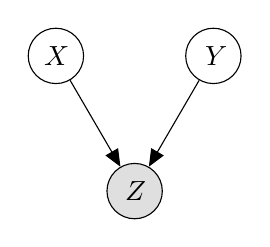
\begin{tikzpicture}
            \node[obs] (z) {$Z$};%
            \node[latent,above=of z,xshift=-1cm,fill] (x) {$X$}; %
            \node[latent,above=of z,xshift=1cm] (y) {$Y$}; %
            \edge {x,y} {z}
        \end{tikzpicture}
        }
        \DisplayProof
        \AxiomC{$X \perp Y \mid Z$}
        \RightLabel{Fork}
        \UnaryInfC{
        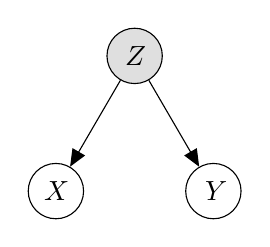
\begin{tikzpicture}
            \node[obs] (z) {$Z$};%
            \node[latent,below=of z,xshift=-1cm,fill] (x) {$X$}; %
            \node[latent,below=of z,xshift=1cm] (y) {$Y$}; %
            \edge {z} {x,y}
        \end{tikzpicture}
        }
        \DisplayProof
        \AxiomC{$X \perp Y \mid Z$}
        \RightLabel{Chain}
        \UnaryInfC{
        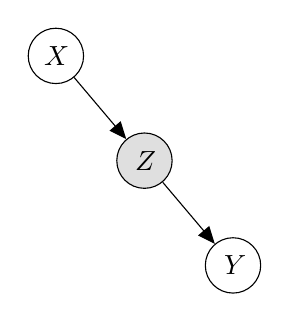
\begin{tikzpicture}
            \node[obs] (z) {$Z$};%
            \node[latent,above=of z,yshift=-11pt, xshift=-32pt,fill] (x) {$X$}; %
            \node[latent,below=of z,yshift=11pt, xshift=32pt] (y) {$Y$}; %
            \edge {x} {z}
            \edge {z} {y}
        \end{tikzpicture}
        }
    \end{prooftree}

    A belief network (BN) is an acyclic DGM of the form:
    \begin{equation*}
        P(x_1,\ldots,x_D)=\prod_{i=1}^D P(x_i \mid \texttt{parents}(x_i))
    \end{equation*}

    Probabilistic graphical models (PGMs) are very expressive, but even approximate inference on belief networks (BNs) is NP-hard~\citep{dagum1993approximating} We can faithfully represent a large class of PGMs and their corresponding distributions as probabilistic circuits (PCs)~\citep{choi2020probabilistic}, which are capable of exact inference in polynomial time and empirically tractable to calibrate using SGD or EM. PCs share many algebraic properties with PGMs and can propagate statistical estimators like variance and higher moments using simple rules.

    Recent work~\cite{choi2020probabilistic} has explored tractable models for probabilistic reasoning based on semiring algebras. Semirings are known to have many useful applications in graph theory~\cite{dolan2013fun} and formal languages~\cite{bernady2013efficient}. A semiring algebra has two operators, $\oplus$ and $\otimes$, with the usual properties. In particular, distributivity holds.

    \begin{prooftree}
        \AxiomC{$X \otimes (Y \oplus Z)$}
        \UnaryInfC{$(X \otimes Y) \oplus (X \otimes Z)$}
        \DisplayProof
        \AxiomC{$(Y \oplus Z) \otimes X$}
        \RightLabel{Distrib}
        \UnaryInfC{$(X \otimes Y) \oplus (X \otimes Z)$}
    \end{prooftree}
    The sum product network (SPN) is a commutative semiring over univariate distributions~\cite{friesen2016sum}:
    \begin{center}
        \begin{tabular}{ccc}
            $PC \rightarrow v \sim \mathcal{D}$ &
            $PC \rightarrow PC \oplus PC$ &
            $PC \rightarrow PC \otimes PC$
        \end{tabular}
    \end{center}

%    Given a BN, we can compile it to a SPN using the following procedure described by~\cite{butz2019sum}:
%
%% Topsort: https://epubs.siam.org/doi/pdf/10.1137/0210049#page=17
%    \begin{algorithm}
%        \begin{algorithmic}
%            \Procedure{Translate}{b: BN}: SPN
%            \State c $\leftarrow $\Call{VariableEliminate}{b}\Comment{Reverse topsort.}
%            \State s $\leftarrow $\Call{RedistributeParams}{c}\Comment{AC $\rightarrow$ SPN.}
%            \State s $\leftarrow $\Call{CompileMarginalized}{s}
%            \State \Return{\Call{Canonicalize}{s}}
%            \EndProcedure
%            \Procedure{Canonicalize}{s$_0$: SPN}: SPN
%            \State s$_1 \leftarrow$ \Call{AddTerminals}{s$_0$}
%            \State s$_1 \leftarrow$ \Call{MergeProducts}{s$_1$}
%            \State $\textbf{if } $s$_0 =$ s$_1$ \textbf{ then return } s$_1$\Comment{Recurse until we}
%            \State $\textbf{else return }$\Call{Canonicalize}{s$_1$}\Comment{reach a fixpoint.}
%            \EndProcedure
%        \end{algorithmic}
%    \end{algorithm}

    \subsection{Knowledge is a graph}\label{subsec:kgs}

    Knowledge graphs~\citep{hogan2020knowledge} are multi-relational graphs whose nodes and edges possess a type. Two entities can be related by multiple types, and each type can relate many pairs of entities. We can index an entity based on its type for knowledge retrieval, and use types to reason about compound queries, e.g. ``Which company has a direct flight from a port city to a capital city?''

    \subsection{Message passing algorithms}

    Many algorithms can be implemented as message passing on graphs...


    \pagebreak\section{From code to procedural knowledge}\label{sec:applications}

    Experts typically encode their knowledge using pen and paper. It is generally possible for skilled coders to translate textual information into code. However there are many equivalent ways to translate text into code -- the same algorithm implemented in the same language by different authors is seldom written the same way. So we need some mechanism to detect exact or approximate equality in procedural knowledge.

    Instead of the Sisyphean task of forever translating these ideas from scratch, coders need to step back and think: Is it possible to just encode the axioms and enough knowledge to derive a family of algorithms, then let the compiler derive the most appropriate procedure for computing some desired quantity? A good compiler might be able to use those facts to optimize computation graphs, e.g. for latency or numerical stability.

    One way to think of big code is as a procedural knowledge system, describing common data transformations and how to achieve them. Suppose we had a \textit{bibliotheca universalis} containing many human-written code examples, which a human could select from manually (a la Hoogle~\citep{james2020digging}) or which could be linked to during compilation. We would like a way to extract common snippets and reason about those transformations, for example to detect similar procedures or optimize an existing procedure.

    Knowledge systems or \textit{ontologies} are a collection of related facts which have been established by human beings. For example, we can treat mathematics as a knowledge base of rewrite rules. This has been successfully operationalized in Theano~\citep{bergstra2010theano}, Kotlin$\nabla$~\citep{considine2019kotlingrad} and other DSLs. More broadly, we can also think of constructive mathematics libraries like Metamath~\citep{megill2006metamath}, Rubi~\citep{rich2009knowledge}, Probonto~\citep{swat2016probonto} and KMath~\citep{nozik2019kotlin} as working towards this same goal.

    In knowledge graphs, approximate equality is known as entity \textit{alignment} or \textit{matching}. With a probabilistic matching algorithm, we could accurately detect near duplicates in a codebase. We could retrieve code samples to assist developers writing unfamiliar code. And we could search for bugs in code or fixes from a knowledge base to repair them. Probabilistic reasoning can be gainfully employed on these and many related tasks.

    Suppose we want to search through a software knowledge base for an error and stack trace, then use the information in the KB to repair our bug.

    \begin{enumerate}
        \item Efficiently searching corpus for a pattern
        \item Identifying alignment and matching results
        \item Incorporating information into user's context
    \end{enumerate}

    \subsection{Code search}

    -model fragments of code and natural language as a graph and learn a distance metric which captures the notion of similarity. Some graphs will be incomplete, or missing some features, others will have extra information that is unnecessary.

    Given a piece of code and the surrounding context (e.g. in an IDE or compiler), search a database for the k most similar graphs, then to recommend them to the user (e.g. fixes or repairs for compiler error messages), or suggest some relevant examples to help the user write some incomplete piece of code. Similar to a string edit distance, but for graph structured objects. There are a few pieces to this:

    \begin{enumerate}
        \item Semantic segmentation (what granularity to slice?)
        \item Graph matching (how to measure similarity?)
        \item Graph search (how to search efficiently?)
        \item Recommendation (how to integrate into user's code)
    \end{enumerate}

    The rewriting mechanism is similar to a string edit distance, but for graphs. One way of measuring distance could be measuring the shortest number of steps for rewriting a graph A to graph B, i.e. the more "similar" these two graphs are the fewer rewriting steps it should take.

    \subsection{Fault localization}

    searching for stack trace on stackoverflow

    \subsection{Program repair}

    adapt some knowledge to match user's context

    \subsection{eDSL generation}

    Take a procedural knowledge base, generate a DSL from it.

    \pagebreak \section{Acknowledgements}

    The author wishes to thank his advisor Jin Guo, Xujie Si and Fuyuan Lyu, for providing several helpful comments on this proposal and Torsten Scholak, David Yu-Tung Hui, Disha Shrivastava, Jordi Armengol-Estap\'e, Matt Rice, Dave Keenan, and John Tromp for various miscellaneous feedback.

    \bibliography{exam_proposal}
    \bibliographystyle{plain}
\end{document}